\chapter{Introduction}
\label{ch:intro}

% \draft{Need to go over with Nicole, probably just writing the intro to an editorial piece, not a thesis.}
% The world has become increasingly urban. Over the last 60 years, global urban populations have grown more than four times; the current urban population (approx. 4,4 billion) is larger than the entire global population in 1975 \cit{https://www.iied.org/urbanising-world}. This growing urban population presents an environmental challenge, although not one usually focussed on. Increasing urbanisation is a benefit for tackling climate change; per capita, urban areas consume less resources and generate less carbon than suburban and rural areas at a similar socio-economic level \cit{holy shit, citation.}. By concentrating human populations, even as they continue to grow, within urban areas, we can mitigate their broader climate impacts. 

% However, increasing urbanisation brings a particular, un-seen environmental challenge: \emph{noise pollution}. 

\section{Background}

Urban noise pollution affects 80 million EU citizens (approx. 20\% of the population) with substantial impacts on public health which are not well addressed by conventional noise control methods \citep{EEA2020Environmental}. Concerns about noise pollution have recently received increased attention both as a global environmental issue \citep{Aletta2022Frontiers} and as a necessary component of the UN Sustainable Development Goals \citep{King2022Here}. Noise pollution has been recognised as the second most impactful environmental health concern in cities, behind air pollution. The WHO found that, among other vectors, transport noise accounted for a loss of 903,000 \glsfirstplural{daly} due to sleep disturbance and 587,000 \glsplural{daly} due to annoyance in the EU \citep{CDC2011Burden}.

Traditional noise control methods have typically limited their focus to the reduction of unwanted noise, ignoring the potential benefits of increasing positive sounds and remaining restricted by practical limitations of noise reduction. Modern approaches to achieve improved health outcomes and public satisfaction aim to incorporate a person's perception of an acoustic environment, an approach known as `Soundscape'\footnotemark.

The soundscape concept represents a positive approach to understanding society's relationship with urban sound. In particular, it stands in contrast to the negative, reactive approach taken in existing noise control regulations. In a recent editorial, \citet{Axelsson2020Soundscape} made this clear:

\begin{quote}
  In practice, noise abatement is a reactive approach to sound. First, a member of the public must submit a complaint to the competent authority, which must verify that the complaint is valid and may then take actions. It is a common view among noise and health inspectors that they have no mandate to act, unless there is a complaint, the validity of which is verified. This makes noise abatement comparable to waste management. Sound is deemed a harmful waste product of human activity that must be removed.
\end{quote}

By contrast, soundscape studies view sound as a resource which both needs to be appropriately managed, but can also contribute positively. Towards this, soundscape studies strive to understand the perception of a sound environment, in context, including acoustic, (non-acoustic) environmental, contextual, and personal factors. These factors combine together to form a person's soundscape in complex interacting ways \citep{Berglund2006Tool}. In order to predict how people would perceive an acoustic environment, it is essential to identify the underlying acoustic and non-acoustic properties of soundscape.

As the future of urban sound research and practice moves toward a more holistic soundscape focus, the ability to affect change at large scales and in a wide range of projects will require that familiar engineering tools and approaches can be applied to soundscape design. When attempting to apply soundscape in practical applications in the built environment, it becomes apparent that a predictive model of the users' perceptual response to the acoustic environment is necessary. Whether to determine the impact of a design change, or to integrate a large scale data at neighbourhood and city levels, a mathematical model of the interacting factors will form a vital component of the implementation of the soundscape approach. 

The ability to predict the likely soundscape assessment of a space is crucial to implementing the soundscape concept in practical design. Current methods of assessing soundscapes are generally limited to a post-hoc assessment of the existing environment, where users of the space in question are surveyed regarding their experience of the acoustic environment \citep{Engel2018Review, Zhang2018Effect}. While this approach has proved useful in identifying the impacts of an existing environment, designers require the ability to predict how a change or proposed design will impact the soundscape of the space. To this end, a model that is built on measurable or estimate-able quantities of the environment would represent a leap forward in the ability to design soundscapes and to assess their broad impacts on health and wellbeing.

It was a combination of research highlighting the health impact of noise \citep{Ising2004Health}, economic impacts of urban noise \citep{Bristow2014International,Galilea2005Valuing} and international-level noise monitoring and mapping efforts which led to the eye-opening statistics showing the true impact of urban noise with which I opened this chapter \citep{EEA2020Environmental}. By creating improved methods and tools which enable the same scale and type of evidence, we can allow research to investigate the full impact of urban sound beyond just its negative, noise-focussed impact, and do so at city- and country-level scales.

% \draft{Need to add a connection here.}

% \section{The SSID Project}
% The \gls{ssid} Project is a five-year, multi-disciplinary project funded by a Horizon 2020 European Research Council grant (no. 740696). The stated goals of the \gls{ssid} project \cit{SSID} were to:

% \begin{quote}
% \begin{enumerate}
%   \item `characterise soundscapes, by capturing soundscapes and establishing a comprehensive database, which will be a cornerstone for the proposed analysis, and an invaluable resource for scientists for years to come.'
%   \item `determine key factors and their influence on soundscape quality based on the database'
%   \item `develop, test, and validate the soundscape indices, through analysing the influences by various factors, using a number of inter- \& trans-disciplinary approaches.'
%   \item demonstrate the applicability of the soundscapes indices in practice, by establishing frameworks for soundscape prediction, design, and standardisation.'
% \end{enumerate}
% \end{quote}

% Although the \gls{ssid} project is broad, including at least eight associated researchers from a wide array of academic backgrounds over its five-year tenure, the work in this thesis will address aspects of all four of its primary goals. \draft{Expand?}

\section{Research aims \& questions}
This work is intended to identify methods for incorporating contextual and objective information into a useable and interpretable predictive model of urban soundscapes and to develop tools for documenting, analysing, and visualising soundscape assessments. In order to achieve this, a protocol for collecting the multi-level, multi-factor perceptual assessment data has been developed and implemented, resulting in a large soundscape database. Several avenues of investigation are then drawn from the database and addressed throughout this thesis.

The primary research questions are:

\begin{enumerate}
  \item What are the primary acoustic features involved in soundscape perception and what are the driving interactions between acoustic features and soundscape assessment?
  % \item How was the change in urban sound environments as a result of the COVID-19 lockdown reflected in the likely soundscape perception? 
  \item To what extent can a predictive model be used to investigate changes in likely soundscape perception in situations where the actual soundscape cannot be assessed?
  \item What are the design and data requirements of a predictive model of soundscape assessments and how can future work move towards achieving these?
  \item How does the sound source composition in a complex sound environment mediate the interactions between acoustic features and soundscape assessment and how can this effect be simplified and modelled?
  \item What are the non-acoustic, personal factors which influence an individual's perception of the sound environment and to what extent do these factors explain the variance in soundscape assessments? 
  \item How can the inherent variation in soundscape assessments across respondents best be represented and in what ways and to what extent can this analysis of soundscapes be applied to address future urban design challenges? 
\end{enumerate}

\section{Methods}

My work in this thesis was completed as part of the \gls{ssid} project, funded by a Horizon 2020 European Research Council grant (no. 740696). The goal of the \gls{ssid} project is to develop a new index for measuring the quality of soundscapes, including the creation of a large scale database of soundscape assessments \citep{Kang2019Towards}. I began this work by developing a data collection protocol (see \cref{chap:protocol}) and building the large scale database of soundscape assessments focussed on understanding the soundscape perception of urban public spaces. I then make use of the database to develop a predictive modelling approach which can be effectively used in a future engineering context. A key consideration of this is that the model inputs rely only on factors which can be measured, estimated, or themselves modelled and fed into the predictive model. 

Throughout, I draw from a machine learning mindset, focussed primarily on the analysis of a large-scale dataset and aimed towards developing a model which can adequately predict soundscape perception. This is in contrast to a statistical inference approach, where the primary goal is to identify and discuss the underlying statistical relationships in a given model. Instead, my main focus is on building prediction through an iterative process of training and testing, while maintaining interpretability of the model. Throughout this thesis, a \gls{mlm} approach has been developed and progressively improved. Although the key chapters make use of separate datasets or be focussed on different aspects of the multi-dimensional perception of urban soundscapes, underlying each of the studies is an analysis based on \gls{mlm} and a goal towards integrating each of their findings into a final, cohesive model. 

\section{Thesis structure}

In this thesis I present the results of several studies which develop the conceptual and statistical frameworks to enable the prediction and presentation of the soundscape analysis of urban spaces. Portions of \cref{chap:protocol,ch:whostudy,ch:mlmann,ch:lockdown,ch:ProbabilisticPOC} have been published in peer-reviewed academic journals. \cref{ch:whostudy,ch:mlmann}, although written in heavy collaboration with coauthors are based primarily on the \gls{mlm} analysis developed in this thesis.

\begin{figure}
  \centering
  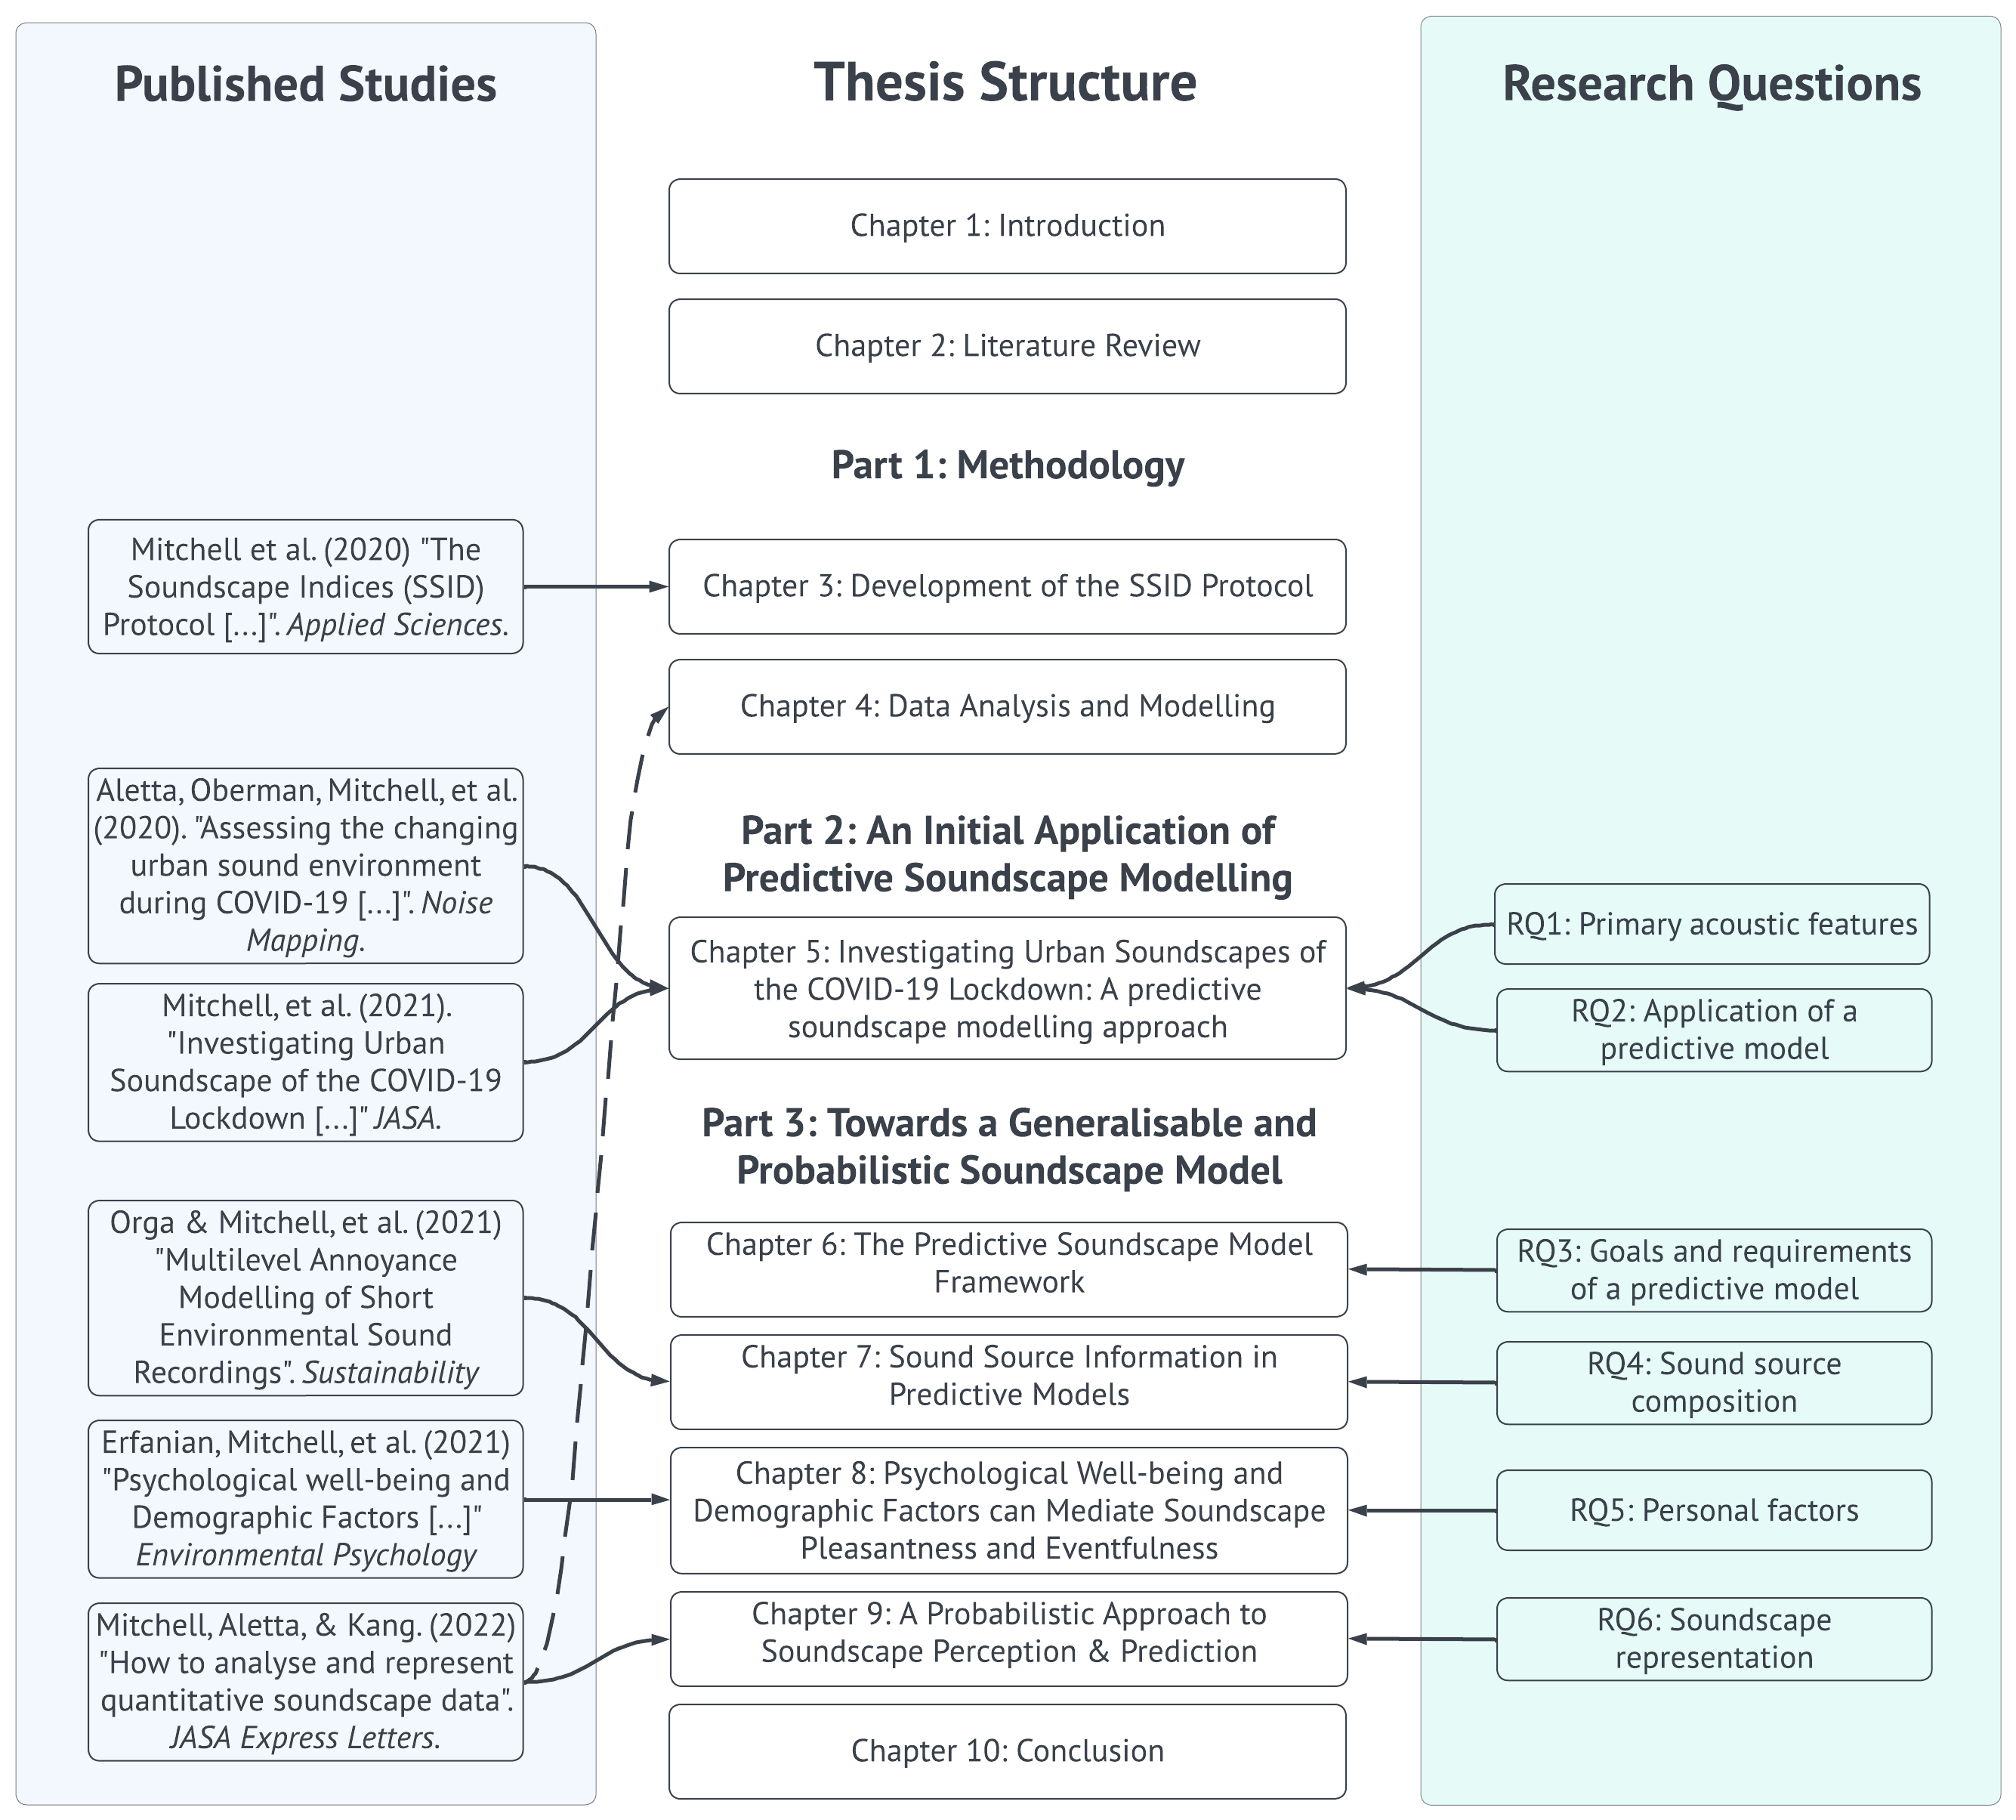
\includegraphics[width=\textwidth]{Figures/Thesis Structure 2022-05-28.png}
  \caption{The overall thesis structure showing how each Research Question (RQ) and published study relates to each chapter. \label{fig:thesisStructure}}
\end{figure}

\textbf{\cref{ch:lit}} begins by reviewing the engineering approach taken in traditional noise control and highlights the improvements offered by the soundscape approach. The current state-of-the-art of soundscape for design is reviewed and the arguments for why predictive modelling is necessary are presented. Finally, the pre-existing framework for predictive soundscape models developed by \citet{Aletta2016Soundscape} and previous examples of predictive models are reviewed. 

After the introduction and literature review, the body of the text containing the original work is separated into three parts: \textbf{\cref{part:Methodology}} contains the methodology; \textbf{\cref{part:Lockdown}} presents an initial development and application of a soundscape model; and \textbf{\cref{part:generalModel}} further develops this initial model with two related modelling studies with discussions of how each of these developments can be integrated into a single, general model. \cref{fig:thesisStructure} presents an overview of the chapter structure of this thesis and how each published study and research question are integrated into the structure.

The methods section is split into two chapters: the first (\textbf{\cref{chap:protocol}}) provides an in-depth explanation of the unique data collection protocol developed for the \glsfirst{ssid} Project and this thesis. The collection and organisation methods included in this protocol were directed toward the creation of a large scale database suitable for training a soundscape prediction model which includes both acoustical and contextual information. The second part of the methods section (\textbf{\cref{chap:methods}}) focusses on how this database is analysed, which includes the questionnaire analysis methods and the multi-level modelling strategy employed throughout the rest of the thesis.

\textbf{\cref{ch:lockdown}} details the development of a predictive soundscape model based on a multivariate psychoacoustic analysis of the collected database. To demonstrate the usefulness of predictive models, this initial model was applied to answer how the soundscape perception of urban public spaces was likely affected by the \gls{covid19} lockdowns in 2020. This chapter begins with an analysis of the sound environment impacts of the lockdowns, as revealed by the psychoacoustic analysis of binaural recordings. An initial \gls{mlm} to predict soundscape pleasantness and eventfulness was trained on data collected before the lockdowns (in 2019) according to the protocol set out in \cref{chap:protocol}, then applied to recordings taken in the same spaces during the height of the 2020 lockdowns (where traditional soundscape assessment methods are impractical) to investigate how these changes to the sound environment would likely have been perceived. 

Following this initial application of soundscape prediction, \cref{part:generalModel} presents several studies which attempt to expand on the initial model. \textbf{\cref{ch:bayes}} begins by laying out a framework of the goals and constraints on a general soundscape model, which was derived from the experience gained in \cref{ch:lockdown}. These goals and constraints establish a series of improvements which can be made to the initial model to move it towards being a useful tool for soundscape design in engineering contexts. 

\textbf{\cref{ch:mlmann}} is the first of these development studies and attempts to integrate sound source information into a psychoacoustic model of annoyance. By collaborating with the DYNAMAP project to use their separate dataset which contains sound-source-labelled recordings from a \gls{wasn}, we investigated the potential for incorporating sound source information in predictive soundscape models and further discuss how this should contribute to a general model. \textbf{\cref{ch:whostudy}} is the second case study and investigates to what degree personal factors (demographics and psychological well-being) influence soundscape perception. This study provides the basis for a consideration of how or whether these factors are necessary for predictive modelling.

Finally, \textbf{\cref{ch:ProbabilisticPOC}} reflects on the analysis methods for soundscape assessment data provided by \citet{ISO12913Part2} and presented in \cref{chap:methods}. Building on the lessons learned in the preceding chapters, I discuss the utility of these methods for describing the soundscapes of public spaces and propose a new analysis and visualisation method that better reflects the variety of experiences that people can have to the same soundscape. The implications of this new conception of a `collective perception' are discussed and proposals for how predictive models should consider this collective perception for the design of public soundscapes are developed.

In all, the results of six peer-reviewed studies are presented. These studies represent a series of work to

\begin{enumerate}
  \item Advance the conceptual development and practice of soundscape studies as applied to public spaces
  \item Develop a transparent and useful method of predicting soundscape assessments
  \item Investigate the various components which influence soundscape perception, including personal factors like psychological well-being, acoustical factors, and sound source specifics and to integrate these components into the predictive modelling methods.
  \item Propose a future framework for predictive soundscape models and provide proposals for how a general model should be developed that can be put to use in engineering approaches to designing the soundscapes of public urban spaces. 
\end{enumerate}

\newpage


\paragraph*{\textsuperscript{1}A note on terminology: Soundscape \emph{Perception}?}

According to the definition of soundscape provided in \citet{ISO12913Part1}, the soundscape is `the acoustic environment as perceived or experienced and/or understood by people'. Both in the standard and elsewhere, this has commonly been taken to mean that the soundscape is the perception itself, while the factors which lead to the soundscape are separate entitites. In this definition, the soundscape is not made up of sound sources, the visual environment, etc. but instead is the perception formed by them. This definition was proposed by \citet{Brown2012review} where the author made this distinction very clear in a section titled \textbf{`Soundscape is perception of the acoustic environment of a place'}: `Thus, a soundscape exists through human perception [\ldots] the soundscape of a place is thus a perceived entity'.

Given this definition, speaking about the `soundscape perception' would be redundant; the soundscape already is the perception. By extension, saying `the soundscape is perceived as pleasant' also would not make sense; we should rather say `the soundscape is pleasant'. However, even among the foundational modern soundscape literature these uses are relatively widespread; \citet{Axelsson2010principal,Liu2014Effects} both refer to soundscape perception within the title.

This definition also conflicts with other popular definitions of soundscape. The term soundscape is commonly used in acoustic ecology and underwater acoustics -- see titles such as `The soundscape of bat swarms' \citep{Kloepper2017soundscape}, `An integrated underwater soundscape analysis in the Bering Strait region' \citep{McKenna2021integrated}, `Soundscape analysis and acoustic monitoring document impacts of natural gas exploration on biodiversity in a tropical forest' \citep{Deichmann2017Soundscape}, and `Identification and quantification of soundscape components in the Marginal Ice Zone' \citep{Geyer2016Identification}. Several analysis packages have also been developed for the purpose of soundscape analysis, whether for urban-, underwater-, or bio-acoustics, which include no aspect of human perception in context (see e.g. Soundscape Viewer \citep{Sun2020Soundscape} and \texttt{scikit-maad} \citep{Ulloa2021scikit}). 

These fields appear to use the term \emph{soundscape} more broadly, without a reference to human perception, to refer to either a broad consideration of the entire sound environment or to a focus on the sound environment as perceived by all creatures, not just humans. This first definition comes from \citet{Pijanowski2011Soundscape} where the authors state that `soundscape ecology focuses mostly on macro or community acoustics [\dots] the
composition of all sounds heard at a location that are biological, geological, or anthropogenic' to differentiate it from previous acoustic ecology studies which `focus on a single species or a comparison of species'. Within the ISO 12913 framework, this would more accurately be described as the \emph{acoustic environment} (`sound at the receiver from all sound sources as modified by the environment'). In the end, all of these conflicting and overlapping definitions can make cross-disciplinary communication more difficult and prone to disagreements and misunderstandings. \draft{I will add approx. 1-2 more paragraphs laying out my definition of soundscape here.}